\chapter{Suffix arrays}\label{ch:suffix-arrays}
Een tweede datastructuur die we in meer detail bekijken zijn suffix arrays.
We kiezen voor deze datastructuur verder te besturderen omdat ze geheugenefficiënter is dan een suffixboom, en bij deze datastructuur hebben we vastgesteld dat het geheugengebruik problematisch is.


\section{Wat zijn suffix arrays?}\label{sec:wat-zijn-suffix-arrays?}
Suffix arrays zijn een geheugenefficiëntere voorstelling van suffixbomen.
In plaats van een boomstructuur maken we hier gebruik van een array die de volgnummers van elke suffix in de originele string bevat.
Deze volgnummers worden lexicografisch gesorteerd op basis van de overeenkomstige suffix.
Figuur~\ref{fig:suffixtree_vs_suffixarray} geeft een voorbeeld van een suffixboom en suffix array opgebouwd over de tekst \texttt{acacgt\$}.

\begin{center}
    \texttt{tekst: a|c|a|c|g|t|\$\\index: 0|1|2|3|4|5|6}
\end{center}
\begin{figure}[H]

    \begin{subfigure}[b]{0.6\linewidth}
        \resizebox{\linewidth}{!}{
            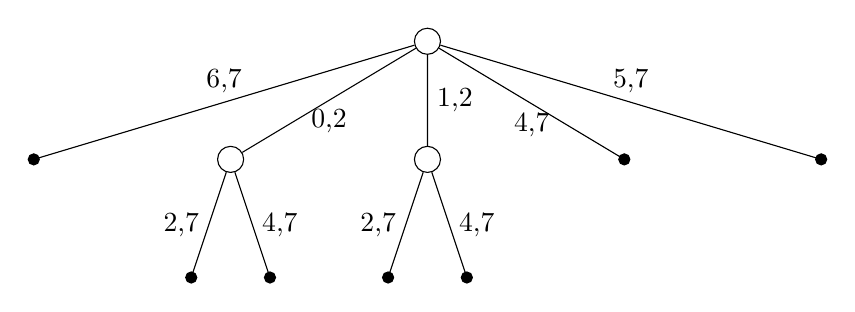
\begin{tikzpicture}
            [
                level 1/.style = {sibling distance = 2.5cm},
                level 2/.style = {sibling distance = 1cm}
            ]

                \node[draw, circle] {}
                child {
                    [fill] circle (2pt)
                    edge from parent node [above] {6,7}
                }
                child {
                    node[draw, circle] {}
                    child {
                        [fill] circle (2pt)
                        edge from parent node [left] {2,7}
                    }
                    child {
                        [fill] circle (2pt)
                        edge from parent node [right] {4,7}
                    }
                    edge from parent node [below] {0,2}
                }
                child {
                    node[draw, circle] {}
                    child {
                        [fill] circle (2pt)
                        edge from parent node [left] {2,7}
                    }
                    child {
                        [fill] circle (2pt)
                        edge from parent node [right] {4,7}
                    }
                    edge from parent node [right] {1,2}
                }
                child {
                    [fill] circle (2pt)
                    edge from parent node [below] {4,7}
                }
                child {
                    [fill] circle (2pt)
                    edge from parent node [above] {5,7}
                }
                ;
            \end{tikzpicture}
        }
        \caption{Suffixboom}
    \end{subfigure}
    \begin{subfigure}[b]{0.4\linewidth}
        \centering
        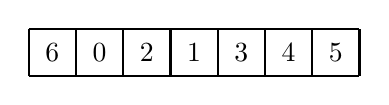
\begin{tikzpicture}[thick,scale=.6]
            \draw (0,0) grid (7,1);
            \path (.5,.5) node{$6$} foreach \i in {0,2,1,3,4,5} {++(1,0) node{$\i$}};
        \end{tikzpicture}
        \vspace{3em} % vertically center the array a bit
        \caption{Suffix array}
    \end{subfigure}

    \caption{Suffixboom en suffix array voor de string \texttt{acacgt\$}.}\label{fig:suffixtree_vs_suffixarray}
\end{figure}

Wanneer we de bladeren van de suffixboom van links naar rechts bekijken dan valt te zien dat dit overeen komt met de suffix array.
Dit is dan ook de link tussen deze twee datastructuren.
Onmiddellijk valt ook te zien dat een suffix array minder data bevat.
De interne knopen uit de suffixboom ontbreken namelijk, samen met de suffix links.
Indien deze informatie ook nodig is kan gebruik maakt worden van zogenaamde Enhanded Suffix Arrays (ESA).
Hierbij worden naast de suffix array nog 3 extra tabellen bijgehouden.
Deze worden de LCP, Child en suffix link table genoemd.


\section{Complexiteit}\label{sec:complexiteit}
Naïef kan het opbouwen van een suffix array in $O(n \log n)$ tijd en $O(n^2)$ geheugen gebeuren waarbij $n$ de lengte van de tekst is, dit aan de hand van traditionele sorteeralgoritmes zoals merge sort~\cite{mergeSort}.
Ondertussen bestaan er echter verschillende algoritmes die een tijdscomplexiteit van $O(n)$ bereiken~\cite{sais, ko_alura, radixSA, dark_archon, libdivsufsort}.
Bovendien vereisen deze veel minder geheugen dan een equivalente suffixboom.
Sommige implementaties vereisen slechts $5n + O(1)$ geheugen~\cite{dark_archon, libdivsufsort} met $n$ de lengte van de invoerstring.


\section{Bestaande implementaties}\label{sec:bestaande-implementaties}
Aangezien er meerdere erg geoptimaliseerde implementaties bestaan voor het opbouwen van een suffix array vergelijken we eerst performantie van deze implementaties.
Op basis hiervan kan daarna beslist worden welke implementatie gebruikt wordt.

\begin{table}[H]
    \begin{minipage}{\linewidth}
        \centering
        \resizebox{\textwidth}{!}{
            \begin{tabular}{l l S[table-format=-2.2] S[table-format=-2.2] S[table-format=-1.2] S[table-format=-1.2]}
                Algoritme & Programmeertaal & \multicolumn{2}{c}{Tijd (in sec)} & \multicolumn{2}{c}{Geheugen (in GB)} \\
                \hline\hline
                &                      & {32 bit} & {64 bit} & {32 bit} & {64 bit} \\
                \cline{3-6}
                libdivsufsort\footnote{\url{https://github.com/y-256/libdivsufsort}}                                       & C                    & 15.01    & 15.97    & 1.03     & 1.86     \\
                libdivsufsort\footnote{\url{https://github.com/baku4/libdivsufsort-rs}}                                    & Rust + bindings to C & 16.00    & 15.52    & 1.03     & 1.86     \\
                libdivsufsort\footnote{\url{https://github.com/fasterthanlime/stringsearch/tree/master/crates/divsufsort}}  & Rust                 & 20.23    & {-}      & 1.03     & {-}      \\
                dark archon a4\footnote{\url{https://github.com/kvark/dark-archon}}                                        & C                    & 39.34    & {-}      & 1.09     & {-}      \\
                libsais\footnote{\url{https://github.com/IlyaGrebnov/libsais}}                                             & C                    & 6.38     & 6.46     & 1.03     & 1.86     \\
                radixSA\footnote{\url{https://github.com/mariusmni/radixSA64}}                                             & C++                  & 9.74     & 11.26    & 2.11     & 3.52     \\
                \hline % TODO: de 2 gewone sais implementaties zijn hier nog niet vermeld, maar is ook niet direct een meerwaarde waarschijnlijk?
            \end{tabular}
        }
        \caption{Uitvoeringstijden en maximaal geheugenverbruik voor het opbouwen van een suffix array aan de hand van verschillende algoritmes voor de Swiss-Prot eiwitdatabank.
        Indien er een 32 bit en 64 bit integer implementatie beschikbaar was werden deze allebei getest. Een - staat voor niet getest. Deze testen werden lokaal uitgevoerd op een laptop. De specificaties hiervan zijn terug te vinden in tabel~\ref{tab:macbook_hardware}.}
        \label{tab:sa_building}
    \end{minipage}
\end{table}

Aan de hand van tabel~\ref{tab:sa_building} kunnen we concluderen dat de meest performante algoritmes op vlak van geheugengebruik libdivsufsort en libsais zijn.
Hierbij is er amper verschil in uitvoeringstijd tussen de 32 en 64 bit versies.
In het algemeen zijn de 64 bit versies een fractie trager.
Bovendien valt ook te zien dat het verschil tussen de C versie en Rust versie die bindings heeft naar de C code klein is.
De overhead van het oproepen van de C code uit Rust is dus minimaal.
Tot slot is libsais voor ons geval het algemeen beste algoritme.
Het geheugengebruik is minimaal en het is bovendien duidelijk het snelste algoritme.
Bovendien bevat het ook een implementatie dat gebruik maakt van 64 bit integers.
Dit is erg belangrijk voor het indexeren van UniprotKB aangezien omdat de totale tekst langer is dan de maximale 32 bit integer.
Dit zorgt ervoor dat alle 32 bit integer implementaties onbruikbaar zijn voor dit einddoel.

\section{Toepassen van suffix arrays op een eiwitdatabank}\label{sec:toepassen-van-suffix-arrays-op-een-eiwitdatabank}
Het moeilijkste stuk van onze probleemstelling is het opbouwen van de suffix array.
Dit stuk kunnen we oplossen aan de hand van de algoritmes beschreven in sectie~\ref{sec:bestaande-implementaties}.
Eens we die suffix array opgebouwd hebben blijft er echter nog een stuk van ons probleem over.
Om te beginnen moeten we nog een mapping maken van de gevonden suffixen naar de bijbehorende proteïnes.
Op basis daarvan wordt daarna de LCA gezocht.

\subsection{Bouwen van de suffix array}\label{subsec:bouwen-van-de-suffix-array}
Zoals in de inleiding in sectie~\ref{sec:probleemstelling} willen we gebruik maken van Rust vanwege de combinatie van \textit{memory safety} en hoge performantie.
We willen echter gebruik maken van de hoge performantie die al verkregen is in sterk geoptimaliseerde, bestaande implementaties van algoritmes op een suffix array op te bouwen.
Daarom hebben we gekozen om gebruik te maken van de interoperabiliteit die bestaat tussen Rust en C/C++ code.
Om het ontwikkelen te beginnen hebben we er voor gekozen om gebruik te maken van bestaande Rust bindings\footnote{\url{https://crates.io/crates/libdivsufsort-rs}} naar de originele C implementatie van libdivsufsort~\cite{libdivsufsort}.
Ook al bleek uit het testen dat dit algoritme voor het opbouwen van de indexstructuur over een eiwitdatabank niet het snelste was, het geheugengebruik is wel minimaal.
\\ \\
Als tweede optie is er voor gekozen om zelf ook een simple Rust wrapper te schrijven rond de libsais C code.
Dit gebruik makende van het \texttt{bindgen}\footnote{\url{https://crates.io/crates/bindgen}} crate.
Op deze manier is het ook mogelijk om met weinig extra code gebruik te maken van deze snellere implementatie.
\\ \\
Het nadeel van het gebruiken van deze bindings naar C code is dat het oproepen van de effectieve C code gebeurd in een \texttt{unsafe} blok.
Hierbij is het dus mogelijk dat er geheugenfouten in het programma sluipen.
Dit risico is echter miniem aangezien dit vrij populaire, geteste bibliotheken zijn.
Bovendien zijn we ook zeker dat als een geheugenfout gebeurd dat dit aan de basis ervan zal liggen.
Dit is dus een afweging tussen optimale performantie (waar het wiel niet heruitgevonden wordt), en garantie van \textit{memory safety}.

\subsection{Mapping van suffix naar proteïne}\label{subsec:mapping-van-suffix-naar-proteine}
Deze mapping kan op twee manieren gebeuren.
Een eerste optie is om expliciet voor elke suffix bij te houden bij welke proteïne die hoort.
Dit kan aan de hand van een array die even lang is als het aantal suffixen.
Het voordeel van deze aanpak is dat het vinden van de bijbehorende proteïne in $O(1)$ tijd kan.
\\ \\
De tweede optie is om enkel de eerste of laatste suffix per proteïne bij te houden.
Het voordeel van deze aanpak is dat er minder geheugen nodig is.
Er is hier $O(n)$ geheugen nodig met $n$ het aantal proteïnen, waar we bij de eerste aanpak $O(m)$ geheugen nodig hebben, met $m$ de lengte van de totale tekst.
Het nadeel is dan weer dat het vinden van de mapping trager is.
Bij deze implementatie duurt het $O(\log n)$ met $n$ het aantal proteïnes aan de hand van binair zoeken.

\subsection{Berekenen van de LCA}\label{subsec:berekenen-van-de-lca}
Zoals eerder vermeld bevat een suffix array geen informatie over de interne toppen die voorkomen bij een suffixboom.
Dit zorgt ervoor dat het niet mogelijk is om op basis hiervan de LCA van de organismen voor te berekenen voor al deze interne toppen.
In de plaats is dit nu iets dat \textit{on the fly} moet gebeuren tijdens het zoekproces zelf.
% TODO: we kunnen ook gebruik maken van enhanded suffix arrays en dat dan wel proberen doen, maar haalbaarheid daarvan is nog uit te zoeken.


\section{Sparse en compressed suffix arrays}\label{sec:sparse-en-compressed-suffix-arrays}
Om het geheugenverbruik van suffix arrays verder te verkleinen kan er gebruik gemaakt worden van sparse of compressed suffix arrays.
Allebei doen ze in principe hetzelfde, er wordt namelijk slechts een stuk van de originele suffix array wordt bijgehouden.
Het verschil zit in welk stuk bijgehouden wordt.
\\ \\
Sparse suffix arrays (SSAs) bouwen een suffix array op basis van elke k-de suffix van de input tekst.
Bij compressed suffix arrays (CSAs) wordt daarentegen slechts elke k-de waarde van de SA bijgehouden.
Voor beide opties is de populairste manier om het samplen uit te voeren na het opbouwen van de volledige SA.
Hierdoor blijft het maximale geheugenverbruik tijdens het opbouwen identiek aan het gebruik van de volledige SA\@.
Dit is net het punt waar wij ons geheugenverbruik verder willen verlagen.
Gelukkig heeft het gebruik hiervan nog altijd het voordeel dat de uiteindelijke machine die de index zal hosten lagere geheugenvereisten zal hebben.
\\ \\
Het samplen is de meest gebruikte methode omdat er tot op vandaag vanwege de sterk bestaande geoptimaliseerde klassieke SA constructie algoritmes.
Bij sparse suffix arrays is het beste tot nu toe een Monte Carlo algoritme dat $O(n)$ tijd en $O(b)$ geheugen nodig heeft en een Las Vegas algoritme dat $O(n \sqrt{\log b})$ tijd en $O(b)$ geheugen verbruikt.
Hierbij is $n$ de lengte van de tekst, en $b$ het aantal effectief gebruikte suffixes in de sparse SA~\cite{building_sparse_sa}.
Merk op dat er dus wel een lineair Monte Carlo algoritme bestaat.
Hierbij is het dus mogelijk dat we afhankelijk van het gekozen algoritme een foutief resultaat hebben, of geen resultaat hebben.
Voor compressed suffix arrays bestaat er een algoritme dat een tijdscomplexiteit van $o(n)$ heeft in combinatie met $O(n \log \sigma)$ bits aan geheugen~\cite{building_compressed_sa}.
Hierbij is $n$ de tekstlengte en $\sigma$ de alfabetgrootte.
\\ \\
Het grootste nadeel aan deze algoritmes in context van deze thesis is dat er nog geen sterk geoptimaliseerde implementaties bestaan.
Bovendien zal de factor van ingevoegde sparseness in ons geval altijd vrij klein zijn om de zoektijden beperkt te houden (aangezien we werken met een erg grote dataset en vrij korte strings).
Wat de winst in geheugenverbruik net volledig teniet zou kunnen doen.
Er wordt niet beschreven wat de constante factor is in het geheugenverbruik.
Bovendien laat een CSA niet toe om rechtstreeks gebruik makende van de CSA te zoeken, er zijn nog extra hulp structuren nodig.
Wat opnieuw extra geheugen vraagt.
Daarom zijn SSAs interessanter.
Deze laten toe om enkel met behulp van de tekst en de SSA te zoeken.

\subsection{Zoeken in sparse suffix arrays}
Het zoeken in een SSA is erg gelijkaardig aan het zoeken in een volledige SA\@.
Een belangrijke restrictie is echter dat in de SSA geen strings gezocht kunnen worden die kleiner dan of gelijk zijn aan de sparseness factor.
Bovendien heeft deze sparseness factor ook een erg belangrijke impact op de zoekperformantie.
Bij het zoeken met sparseness factor $k$ moeten we namelijk alle suffixen zoeken die matchen met de gezochte string waarbij we eerst $p \in [0, k-1]$ tekens overslaan.
Voor elke matchende suffix moet daarna gecontroleerd worden als de overgeslagen prefix van $p$ tekens matcht met de $p$ tekens voor gematchte suffix (stel dat dit suffix $s$ is).
Als dit zo is, dan matcht suffix $s-p$ met de gezochte string.